\chapter{Refactoring}
In diesem Kapitel sollen die Refactorings betrachtet werden.
    \section{Identifizieren von Codesmells}
    Hierbei wurde das Sonar Lint Plugin verwendet, um die bestehenden Code-Smells des Projektes anzuzeigen. Dabei wurden die gefundenen Fehler mit den RISC Nummern abgeglichen, um einen Lösungsansatz zu bekommen.
        \subsection{Codesmell 1}
        \begin{figure}[h]
        	\centering
        	%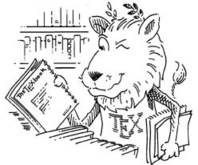
\includegraphics[height=150px]{./appendix/filesONLYForAppendix/Images/lion.png}
        	\shadowimage[height=80px]{./zfiles/Bilder/CodeSmell.png}
        	\caption{Codesmell 1 - Unnötige Imports löschen}
        	\label{codesmell_1}
        \end{figure}
        Der erste Codesmell befasst sich mit den bei der Entwicklung importierten Bestandteilen. Bei der Entwicklung werden oft verschiedene Packages importiert, die wegen Codeänderungen am Ende gar nicht verwendet werden. Dieser Code-Smell mit der Kennung \hk{java:S1700} soll nun behoben werden. 
        \subsubsection{Begründung}
        Diese Imports stellen ein Sicherheitsrisiko für die Anwendung dar und tragen außerdem nicht zur besseren Lesbarkeit des Codes bei, deshalb sollen sie entfernt werden.
        \subsubsection{Fix}
        Diese Imports müssen schlichtweg aus den implementierten Klassen entfernt werden. Dies kann manuell oder mit dem Refactoring Tool der IDE umgesetzt werden. Dieses Refactoring wurde im Commit \hk{70c0170a518290b3449e383bd04e1c7e99e740fd} umgesetzt.
        
        \subsection{Codesmell 2}
        \begin{figure}[h]
        	\centering
        	%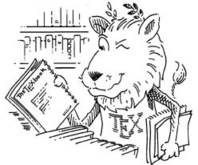
\includegraphics[height=150px]{./appendix/filesONLYForAppendix/Images/lion.png}
        	\shadowimage[height=90px]{./zfiles/Bilder/CodeSmell2.png}
        	\caption{Codesmell 2 - Variablennamen gleich dem Klassennamen}
        	\label{codesmell_2}
        \end{figure}
        Der zweite Codesmell bezieht sich auf die Namen von Variablen in Klassen. Hierbei hieß eine Variable wie die Klasse, in der sie verwendet wurde. Das ist nach java:S17000 ein schwerwiegender Codesmell
        \subsubsection{Begründung}
        Wenn das Attribut wie die Klasse heißt, verwirrt das den Entwicker und sollte neu benannt werden.
        \subsubsection{Fix}
        Umbenennung des Attributes wurde in Commit \hk{d4bb6279cfc335f8967256a795db978ae6ad6930} umgesetzt.